
\documentclass[12pt,a4paper]{article}
\usepackage{listings}
\usepackage[usenames,dvipsnames]{color}
\usepackage{graphicx}
\usepackage{subfig}
\usepackage[margin=1in]{geometry}

\author{Sebastien Duc}
\date{\today}
\title{$2^{\mathrm{st}}$ mini project - K-means}

\begin{document}
\maketitle
\definecolor{orange}{rgb}{1,0.5,0}
\lstset{language=python,keywordstyle=\color{orange},commentstyle=\color{blue},basicstyle=\footnotesize}
\section*{About the project}
To run the project, type \texttt{python kmeans.py}. Note that convergence can take some time. There is just one python file. All functions needed for this project are in this file.
There are 3 main functions. The first is \texttt{normal(improved)} which takes \texttt{improved} (a \texttt{Boolean}) as parameter. This is used for the first part of the project.
When \texttt{improved = False}, the vanilla $k$-means is used on the data set. When \texttt{improved = True}, the dead unit reducing version is used.

The second function is \texttt{reduced(improved)} which takes again a \texttt{Boolean} as parameter. This function is used for part 1.1. It first reduces the data set using PCA and 
then applies $k$-means on it. Again \texttt{improved} allows us to choose between the standard and the improved version of the algorithm.

The third function is \texttt{blind(reduction)}. \texttt{reduction} is either \texttt{None}, in that case we do not reduced the data set before applying $k$-means. Or 
\texttt{reduction} is an \texttt{Int}, in that case we reduce the data set by keeping only \texttt{reduction} dimensions and then apply $k$-means.

\section*{Part 1.1}
\subsection*{The basic algorithm}
The algorithm used for this project is the batch version of $k$-means.
First we initialize the prototypes with random elements from the data set. Then, while the clusters have not converged, first we assign for each data element of the data set
the closest prototype. Then we update the prototypes using the batch rule
\[
\mbox{For each prototype $p$ that represent cluster $C_p$} \quad p \leftarrow p + \mu \sum_{e \in C_p}{p - \mathrm{DataSet}[e]}
\]
The criterion of convergence we used is the number of data elements of the data set that changes cluster. If no data elements changed cluster then we say that the algorithm has converged.
See Figure~\ref{fig:convergence} to have a plot of the time course of our convergence measure.
\begin{figure}
    \centering
    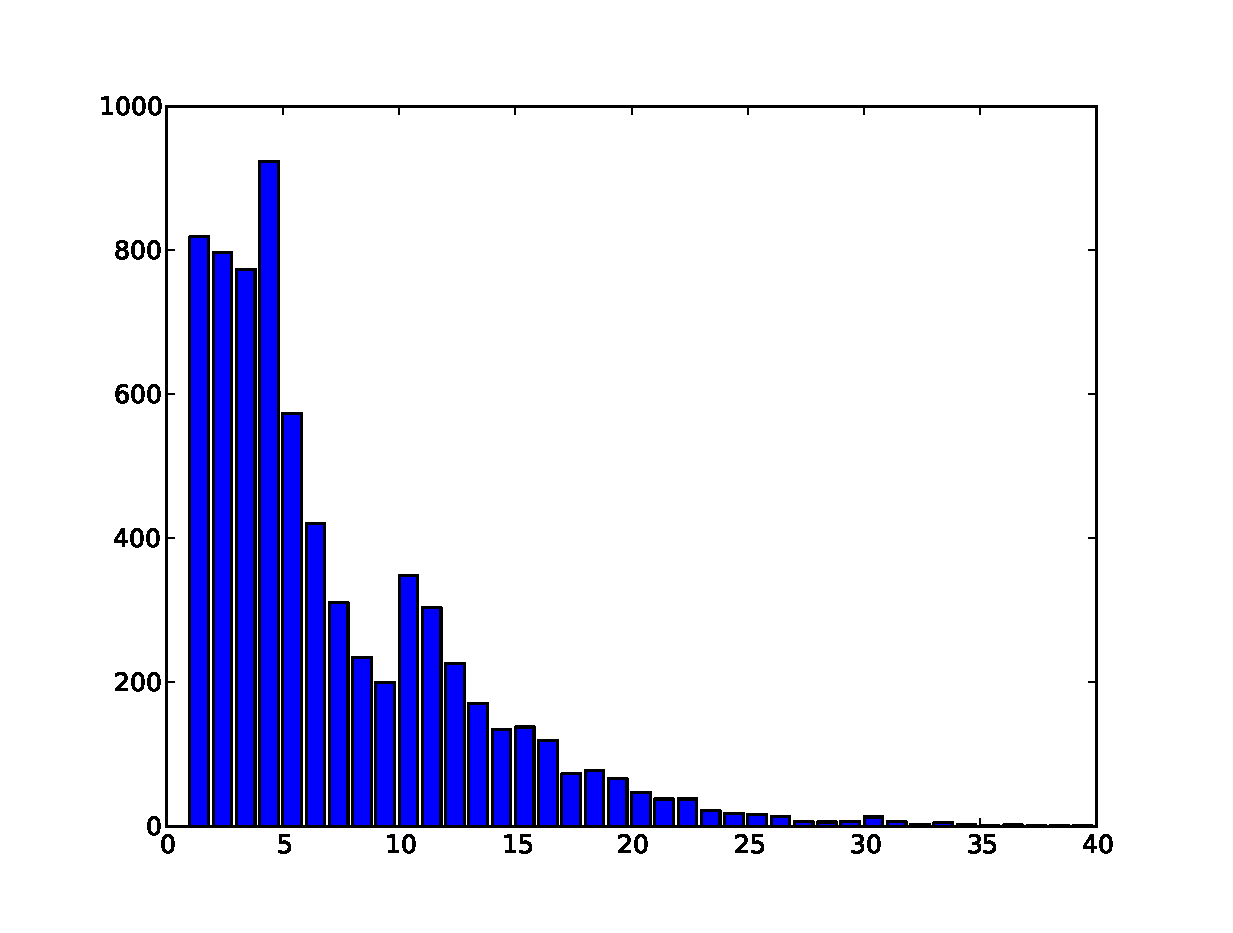
\includegraphics[width=0.5\textwidth]{convergence}
    \caption{Time course of convergence measure}
    \label{fig:convergence}
\end{figure}

For the prototypes, see Figure~\ref{fig:proto1.1}. To get all the digit, $k = 10$ is not enough because some clusters represent the same digit. With $k=20$ we have most of the time
all digits.
\begin{figure}
    \centering
    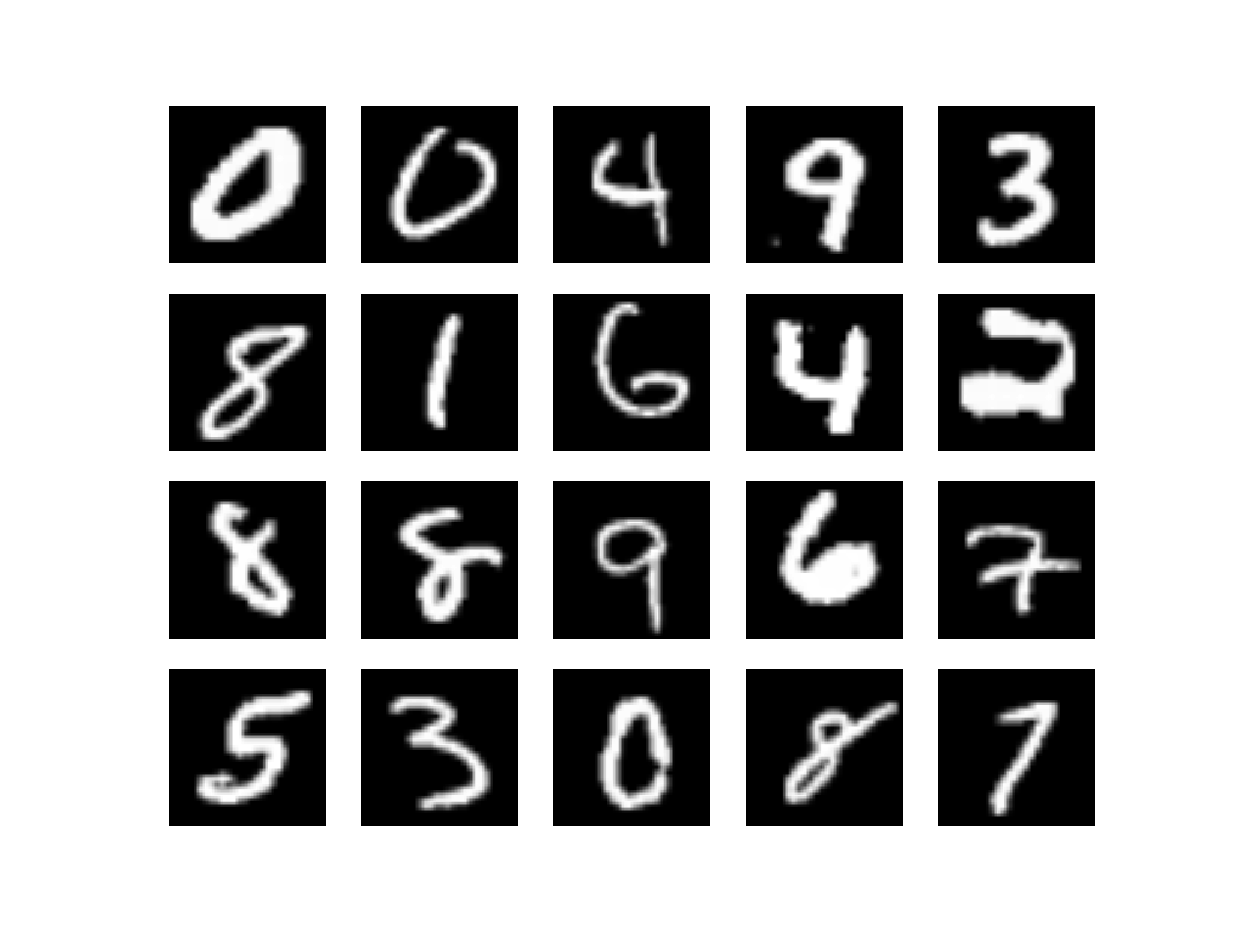
\includegraphics[width=0.5\textwidth]{proto1}
    \caption{Prototypes with $k=20$}
    \label{fig:proto1.1}
\end{figure}

To detect dead units, we look at the number of data elements that are in the cluster. If this number is less than some threshold (for example 50), then we say that it is a dead unit.
Dead units appear only when $k$ is big. 

We also computed the shannon entropy of the clusters, but we need to have the label to do this.  The entropy is computed as following: 
for each cluster $C$ find the number of data elements $n_i$  with label $i$ (i.e. that represent digit $i$) normalize them ($p_i \leftarrow \frac{n_i}{\sum_i{n_i}}$). 
Then $H(C) = \sum_i{p_i \log\frac{1}{p_i}}$. A low entropy means that the cluster represent 
a single digit and a high entropy means that the cluster represent a mix of digits.
\subsection*{The improved algorithm}
The purpose of this new version is to avoid dead units. To achieve this, we changed a bit the initial algorithm.
First each time we update the clusters, we assign with low probability the data element to a random cluster. Also, we decrease the learning rate $\nu$. 

We also tried to improve the initialization, so that the initial prototypes are far away for each other. For the first prototype, pick one data element at random. Then pick a next 
data element with probability proportional to the square of the distance to the nearest prototype already chosen until we have $k$ prototypes. This method didn't really increased the
preformances. When doing statistics on 20 trials, we got on average 2.5 dead units for the initial algorithm and 2.0 for the improved one. 

To detect clusters that represent the same class, we can compute the correlation matrix of the prototypes. A high correlation means the the clusters represent the same cluster.

\section*{Part 1.2}
In this part we reduced the size of the data set. First we kept only data with label 0,1,2,3. And then we applied PCA on this set, by keeping only 4 dimensions. 
In Figure~\ref{fig:reduced} we plotted some subsets of the 4-dimensional reduced set. Label 0 is in red, label 1 in blue, label 2 in green and label 3 in yellow.
One can clearly see some clusters in these plots.
\begin{figure}
    \centering
    \subfloat{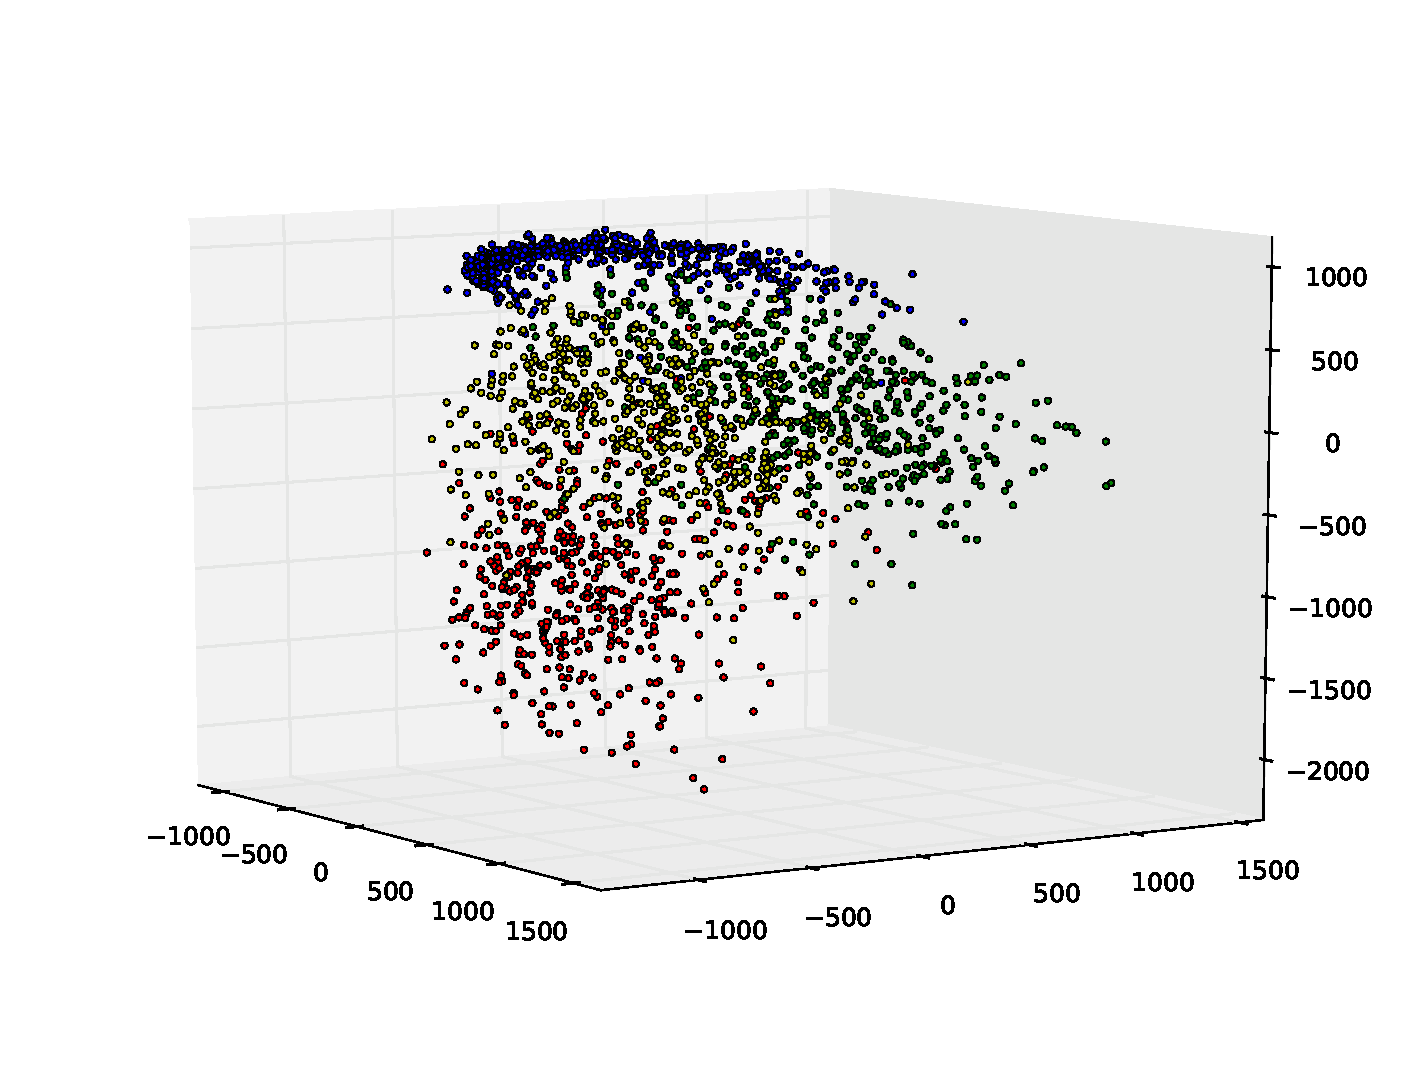
\includegraphics[width=0.3\textwidth]{reduced}}
    \subfloat{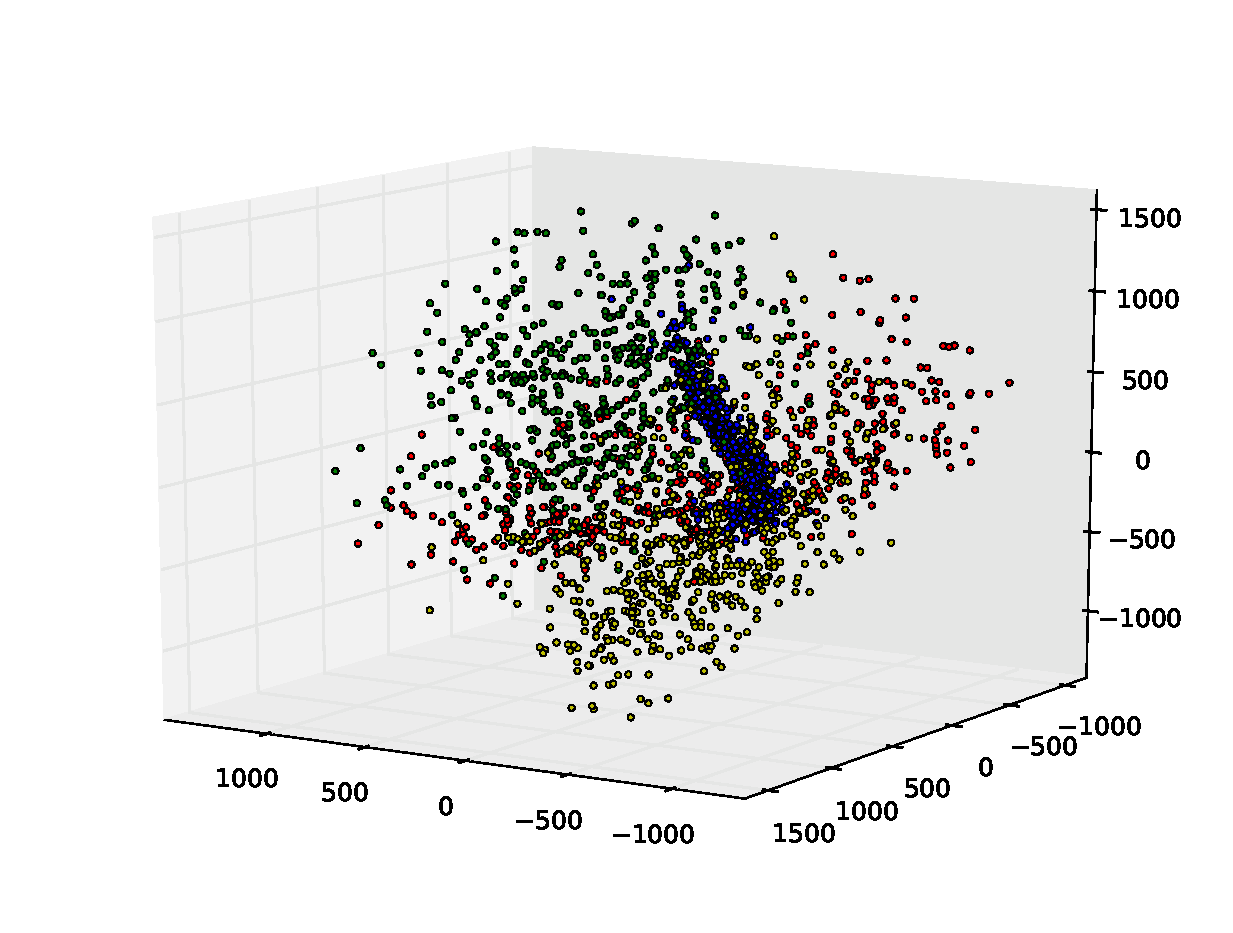
\includegraphics[width=0.3\textwidth]{reduced012}}
    \subfloat{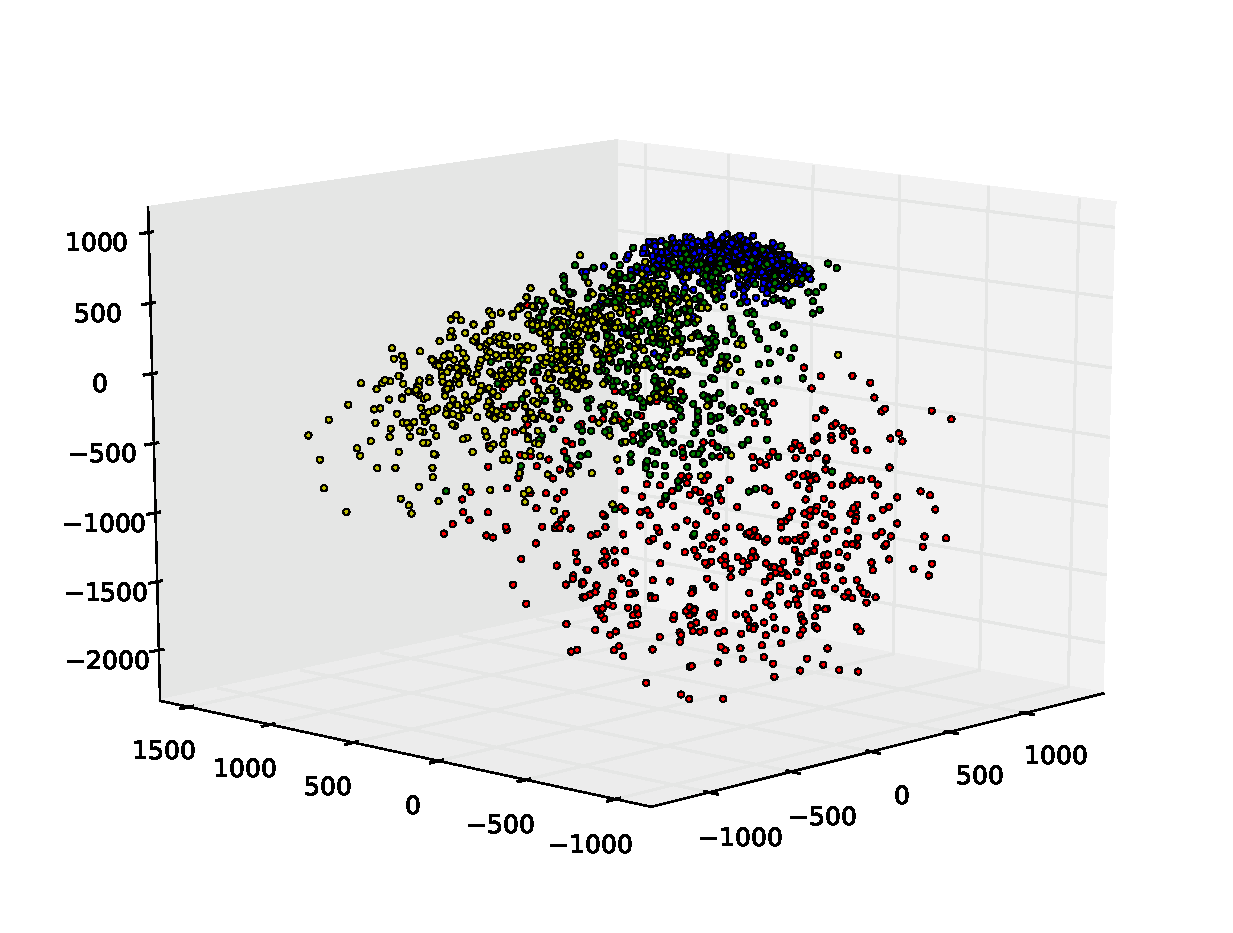
\includegraphics[width=0.3\textwidth]{reduced013}}
    \caption{Subsets of the data set after PCA}
    \label{fig:reduced}
\end{figure}

Then when we apply $k$-means on this reduced set we get 4 by 4 digit pictures. One can see them in Figure~\ref{fig:reduced_proto}
\begin{figure}
    \centering
    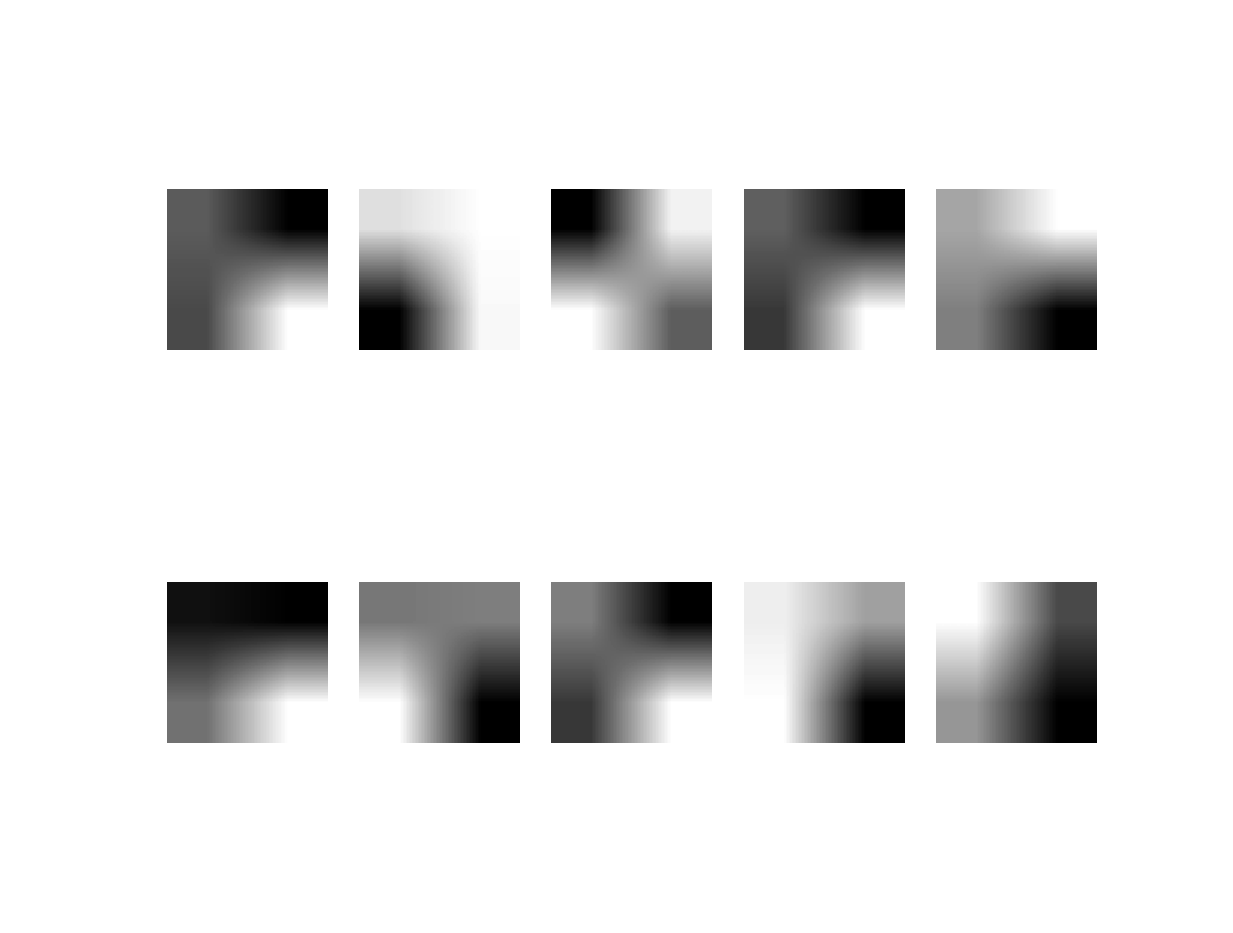
\includegraphics[width=0.5\textwidth]{reduced_proto}
    \caption{Reduced prototypes with $k=10$, and keeping 4 dimensions}
    \label{fig:reduced_proto}
\end{figure}
Then we also applied $k$-means on the reduced set but keeping 25,64 and 400 dimensions. One can see the prototypes in Figure~\ref{fig:reduced_proto_dim}.
\begin{figure}
    \centering
    \subfloat[Dimension is $5\times 5$]{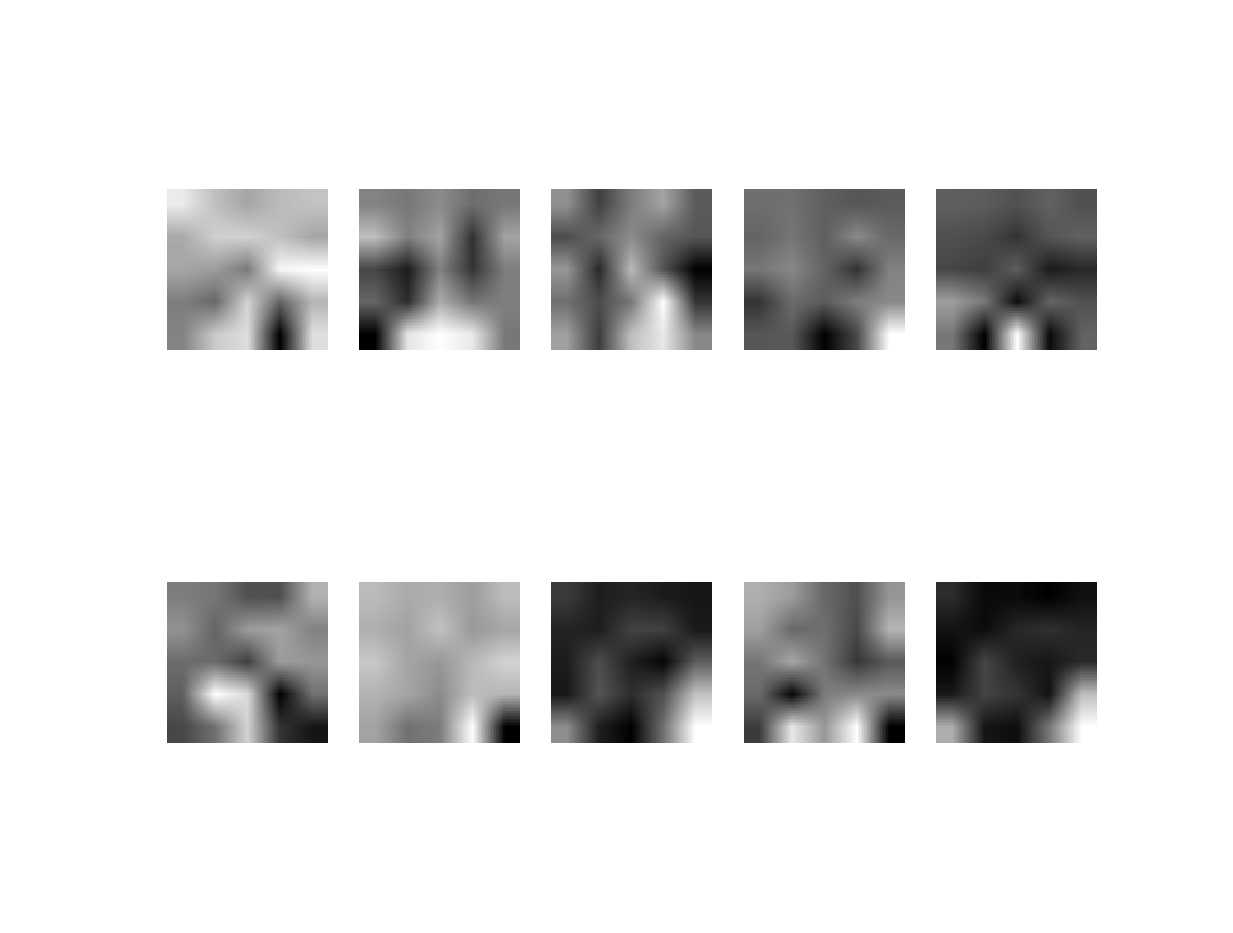
\includegraphics[width=0.3\textwidth]{reduced_proto5}}
    \subfloat[Dimension is $8\times 8$]{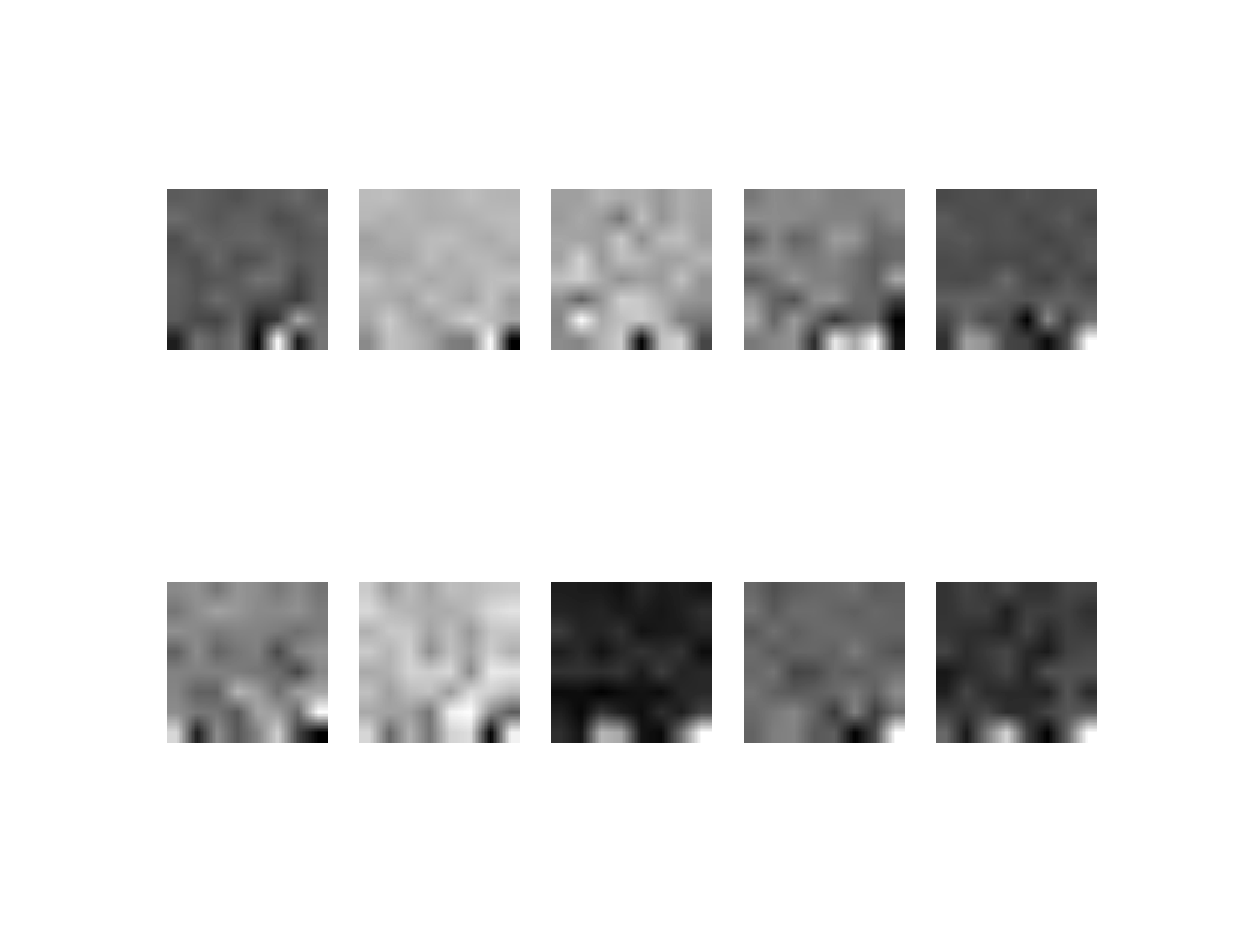
\includegraphics[width=0.3\textwidth]{reduced_proto8}}
    \subfloat[Dimension is $20\times 20$]{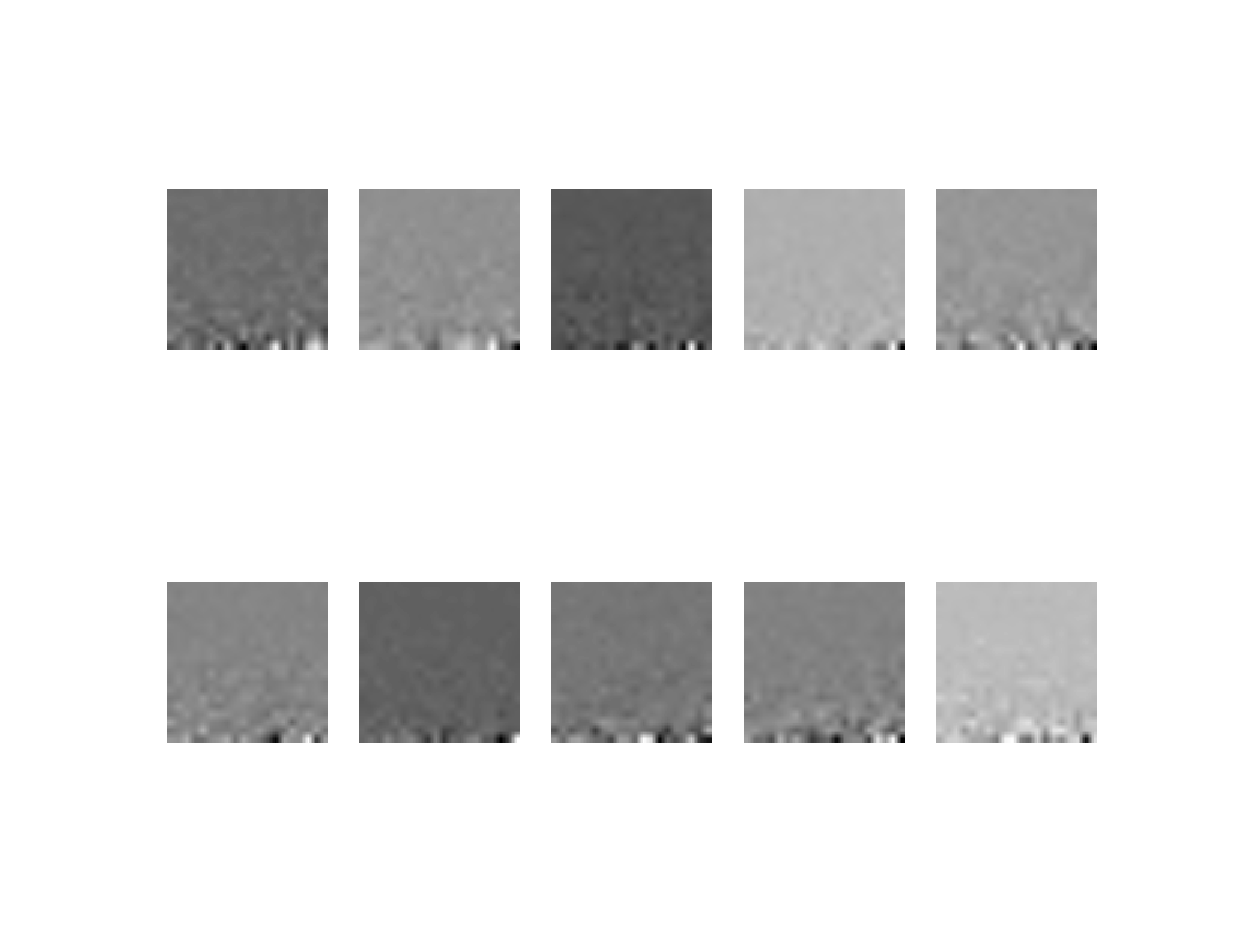
\includegraphics[width=0.3\textwidth]{reduced_proto20}}
    \caption{Reduced prototypes with $k=10$, and keeping 25,64,400 dimensions}
    \label{fig:reduced_proto_dim}
\end{figure}

\section*{Part 2.1}
The prototypes are available in the file \texttt{blindprototypes.txt}. The algorithm was run with $k=20$. The prototype 7 is probably a dead unit
\end{document}
